\documentclass{beamer}
\usepackage[style=authortitle-comp]{biblatex}
\usepackage[export]{adjustbox}

\title{Progress Report: Page Cache Consistency Model}
\author{Zhengyi Chen}
\date{\today}

\addbibresource{../main.bib}

\begin{document}
% Title page
\frame{\titlepage}

% Page 1
\begin{frame}
    \frametitle{The System}
    \begin{itemize}
        \item Remote node(s) abstracted as shared memory device ``\texttt{/dev/rshm}''
        \item {
            Heterogeneous Memory Management (HMM) ensures unified address space between
            local and device memory.
        }
        \item {
            Migration of pages between CPU and ``device'' is transparent to userspace
            -- no need for copying/mapping.
        }
        \item {
            In reality, ``\texttt{/dev/rshm}'' a handler for RDMA access between nodes.
            \begin{itemize}
                \item This involves remote read/write and moving page content between nodes.
                \item Local node serves as \emph{home node \& address space host} at share time.
                \item Remote nodes attached on \texttt{/dev/rshm} as accelerator.
            \end{itemize}
        }
    \end{itemize}
\end{frame}

% Page 2
\begin{frame}
    \frametitle{The Problem: Consistency Protocol}
    \begin{itemize}
        \item Single-Writer, Multiple-Reader Protocol
        % Why?
        % It may be that this mimics all sorts of logic for hardware acceleration
        % -- that is, in an HMM node each PCIe device have sole access to a page of memory.
        % For example, during machine learning you naturally can't access the same, say,
        % kernel by both CPU and GPU.
        % That said, I never shed a doubt on this issue except my advisor telling me not
        % to worry about it -- if I was asked this problem for some reason I'd be cooked!
        \item Need to be performant\dots with some ergonomics
        \item {
            Two Hypothetical Protocols:
            \begin{itemize}
                \item ``RwLock'' Consistency Protocol
                \item Acq-Rel Consistency Protocol
            \end{itemize}
        }
        \item {
            Former ensures \emph{strong} single-writer consistency
            \begin{itemize}
                \item -- Also easier to program with!
            \end{itemize}
        }
        \item Latter allows concurrent in-memory \emph{non-committal} computation
    \end{itemize}
\end{frame}

% Page 3
\begin{frame}
    \frametitle{``RwLock'' Consistency Protocol}
    Similar to a read-write lock where:
    \begin{itemize}
        \item Multiple readers can exist for a clean page -- the page is \textbf{shared}.
        \item Only one write is allowed for a clean page -- the page becomes \textbf{exclusive}.
        \item {
            For one writer node to be allowed sole write access to some page, all other
            readers need to have their page cache invalidated.
        }
        \item {
            While the sole writer node has not yet committed, no other reader or writer nodes
            are allowed to be served this page.
        }
        \item {
            When the sole writer commits, it becomes the new home node which serves the
            updated page content.
        }
    \end{itemize}
\end{frame}

% Page 4
\begin{frame}
    \frametitle{``RwLock'' Consistency Protocol}
    \begin{figure}
        \centering
        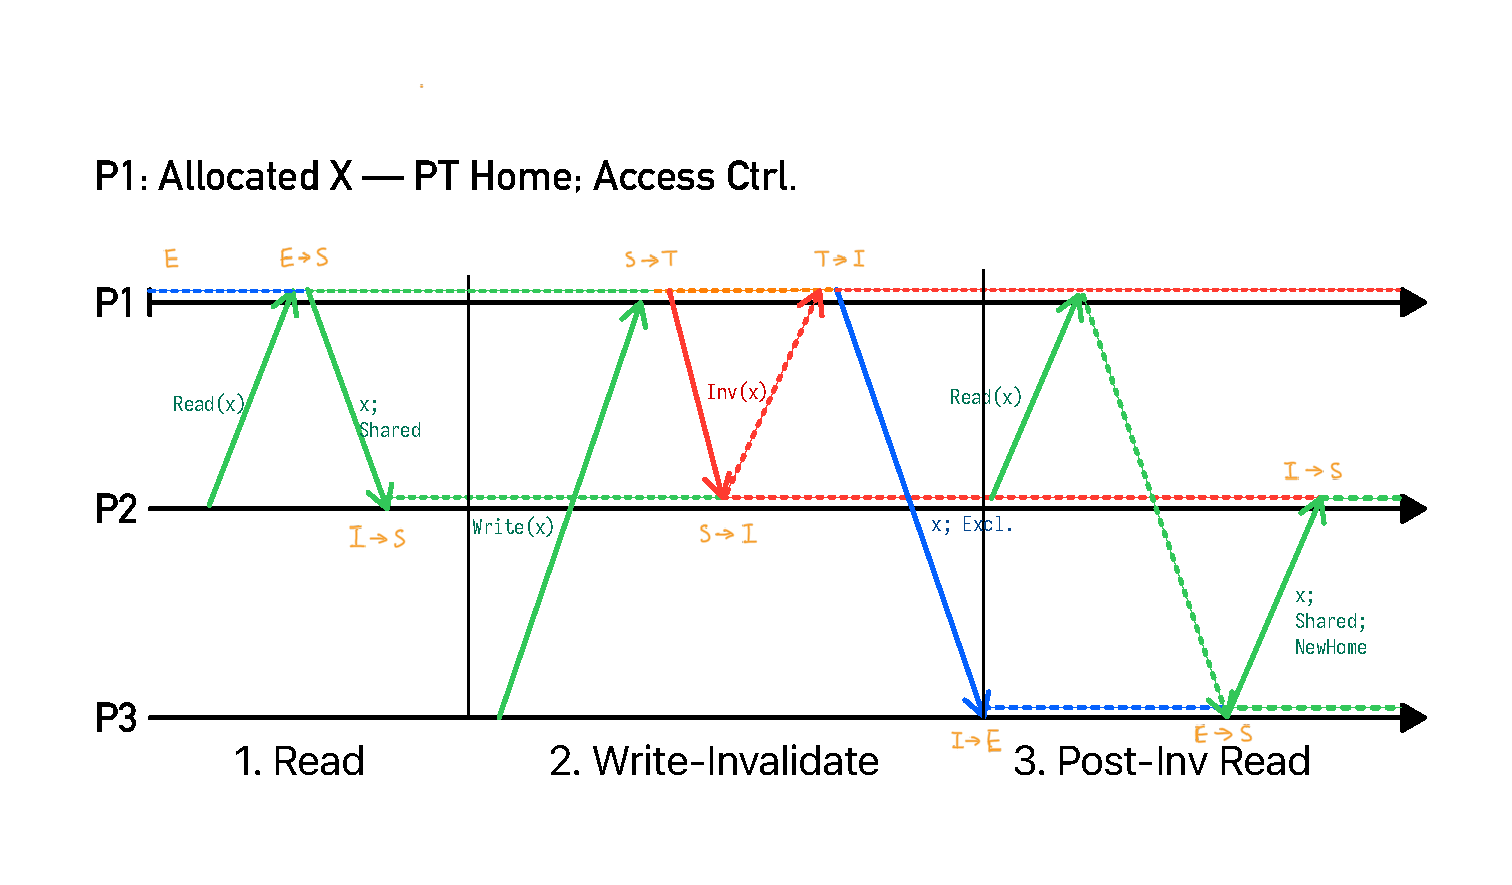
\includegraphics[width=\linewidth]{
            w12_slides_resources/Fig-RwLockProtocol 2023-12-04 21_03_50.pdf
        }
    \end{figure}
    Note: The blue arrow should be acknowledged by P3 -- forgot to put the ack. arrow in.
\end{frame}

% Page 5
\begin{frame}
    \frametitle{Acq-Rel Consistency Protocol}
    In RwLock's case, read requests result in installation of read-only pages at
    remote nodes.

    Alternatively, this protocol allows read/write pages to be installed at remote
    nodes at read time. Such writes are \emph{non-committal} and cannot be synced
    with the entire system.

    To summarize:
    \begin{itemize}
        \item {
            ``Readers'' can write to its locally installed page without any means
            to synchronize the change.
        }
        \item {
            ``Writers'' need to acquire global write access from the \emph{PT node},
            which invalidates all shared pages.
        }
        \item {
            i.e., Instead of write-invalidate, perform acquire-invalidate.
        }
    \end{itemize}
\end{frame}

% Page 6
\begin{frame}
    \frametitle{Consistency Protocol: Knobs and Mods}
    We can modify these two protocols further as follows:
    \begin{itemize}
        \item {
            Multi-home Protocol: instead of having one home at a time, have
            multiple homes (e.g., when writer commits) to prevent network bottleneck.
        }
        \item {
            Auto-share: Mark pages shared via \texttt{/dev/rshm} as automatically
            shared to some remote nodes such that 1-way communications suffice to
            re-validate invalidated pages.
            \begin{itemize}
                \item Potential for communication reduction -- debatable.
            \end{itemize}
        }
    \end{itemize}
\end{frame}

% Page 7
\begin{frame}
    \frametitle{What about Consistency \textbf{Model}?}
    \begin{itemize}
        \item {
            The weaker a consistency model is, the more difficult it is to program with.
            \begin{itemize}
                \item {
                    Weak ordering architectures (e.g., ARMv8) more or less depends on
                    compiler/interpreter to emit barriers as see fit \cite{Haynes_2022}.
                }
                \item {
                    Bad for usability/portability -- programs may need
                    to be compiled using a modified toolchain, else need to add these
                    synchronization instructions/function calls everywhere.
                }
            \end{itemize}
        }
        \item {
            \footcite{cai2018efficient} uses Partial Store Order.
            \begin{itemize}
                \item Preserves RAR, WAR -- ``synchronous read\dots asynchronous write''
                \item Easier to use than relaxed ordering.
            \end{itemize}
        }
        \item {
            \footcite{wang2021concordia} uses strong consistency, but warns about its scalability.
        }
    \end{itemize}
\end{frame}

% Page 8
\begin{frame}
    \frametitle{Consistency Model: Cont.}
    \begin{itemize}
        \item {
            Similar to Concordia\footcite{wang2021concordia}, the proposed protocols also assume
            strong consistency.
        }
        \item {
            Further work needed to see how to adapt these protocols for weaker consistency models.
        }
    \end{itemize}
\end{frame}
\end{document}